\chapter{Computational modelling of tissue ablation}
\label{chap:ablation}
\section{Introduction and background}
Lasers are used in wide variety of medical procedures not limited to: coagulating scalpels, port wine stain removal, tattoo removal, hair removal, and skin rejuvenation~\cite{amini2010ultrafast, tan1989treatment,kuperman2001laser,liew2002laser,hardaway2002nonablative}.
One class of laser used in these procedures are ablative lasers. Ablative lasers are usually high powered lasers targeted at a specific chromophore in the skin, to partially or fully remove layers of skin. These types of lasers are commonly used for aesthetic procedures such as: skin rejuvenation~\cite{hardaway2002nonablative}, and removal of various diseases such as Rhinophyma~\cite{shapshay1980removal} or lesions/nodules~\cite{valcavi2010percutaneous}. They have also recently been investigated as a means of better drug delivery in the skin for \gls{pdt} treatments~\cite{haedersdal2010fractional}.

One downside to using lasers to remove tissue, it that unlike a scalpel, where the surgeon has full control of the depth of the incision, ablative lasers are not as predictable. Lasers can also cause  thermal damage to the surrounding areas, leading to potentially  unwanted effects, though some applications of ablative lasers utilise the thermal damage, particularly aesthetic procedures~\cite{alexiades2008spectrum}.

 Currently the only reliable method to measure the depth of the ablative holes, is via a biopsy, which is an invasive procedure. We propose to use \gls{oct} to measure the ablative crater non-invasively \textit{in-vivo}. The \gls{oct} measurements are then backed up by a computational model. This computational model could be used to predict the depth of the ablative crater when using a certain laser power for various different applications such as: laser assisted drug delivery, and various cosmetic applications.

\medskip

This chapter examines using \gls{mcrt} techniques coupled to a heat transfer simulation, in order to study the thermal damage to tissue due to fractional lasers. Fractionated ablative lasers  are ablative lasers where the power is spread over several beams, such as to leave viable tissue around zones of damaged/necrotic tissue~\cite{manstein2004fractional}. We present experimental work carried out on porcine tissue by our collaborators at the University of Dundee and the photobiology department at Ninewells hospital, along side our computational model of tissue ablation.

\section{Methods}

In order to replicate the experimental work \textit{in silico}, our numerical model has three main portions. The first is the \gls{mcrt} that models light transport through tissue so that we can calculate the laser energy deposited as a function of time and space. The second, a \gls{fdm} which is used to calculate the heat diffusion within the tissue due to the absorbed laser energy. Finally, a tissue damage model to track the tissue damage caused by the laser. All these individual portions are connected together to create our numerical model. This chapter explains in detail each portion of the numerical model used to simulate tissue ablation via a laser.

\subsection{Monte Carlo radiation transport (MCRT)}

*This part is here as it will be needed for paper. probably not needed in chapter though...*
\gls{mcrt} is the `gold standard' for simulating the transport of light through biological tissue~\cite{kong2008efficient,wang1995mcml}. This is due to its flexibility in modelling non-standard geometries, various light sources, and micro-physics, such as fluorescence. It uses interaction probabilities and random numbers in order to model the `random walk' that photons undergo in a turbid medium. We simulate the propagation of photon packets, which represent photons with a given power, derived from the incident radiant source. These `packets' can undergo go scattering, absorption and various other physical process \cite{yao1999monte,welch1997propagation}. \gls{mcrt} has been used to model light-tissue interactions in many different medical and biophotonic applications \cite{campbell2015monte,boas2002three,patwardhan2005monte}. \gls{mcrt} is used here to calculate the energy deposited by the laser, which is then passed to the heat transport simulation.

The original \gls{mcrt} code was developed for astronomy applications \cite{wood1999model,wood2005estimating}, and has since been adapted for medical applications~\cite{campbell2015monte,barnard2018quantifying}.

The tissue medium for the \gls{mcrt} and heat transport simulations is a 3D voxel model (\cref{fig:voxel-model}). This allows the variation of optical and thermal properties from voxel to voxel, making it the ideal type of grid for modelling tissue ablation. We use  160 $\times$ 160 $\times$ 160 voxels, representing a tissue sample size of .06 $\times$ .06 $\times$ .18~$cm$. We assume the porcine skin is uniform, so initially our voxel model is uniform, and the optical properties of porcine skin at the wavelength of interest is mainly that of water mixed with protein, see \cref{fig:waterabsor}.


\begin{figure}
\centering
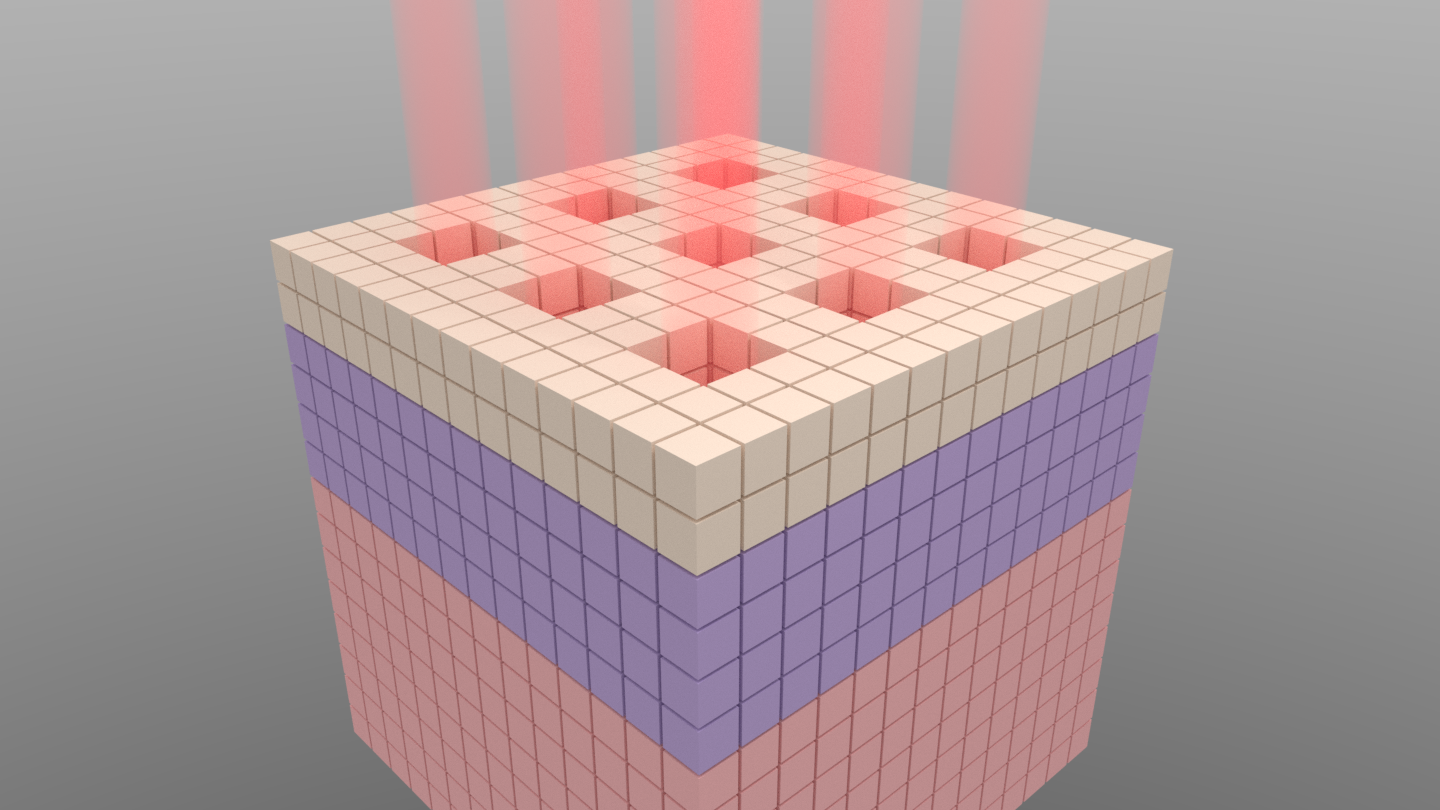
\includegraphics[scale=0.25]{./ablation/images/voxel-model-render.png}
\caption{Example of a possible voxel model, with three different layers, various holes due to ablative pixel beam lasers. Each voxel can represent a different optical/thermal propertty of the tissue medium.}\label{fig:voxel-model}
\end{figure}

\Cref{fig:algo}. shows the overall algorithm for the simulation, including the \gls{mcrt} portion. 
The \gls{mcrt} portion of the algorithm begins with determining where the photon enters the medium. This is calculated by randomly selecting one of the pixel beams, from the 9 x 9 array of pixel beams. Next the position on the surface of the medium is calculated. As the exact profile of the pixel beams are unknown, we assume them to be uniformly circular. Thus, the packets position is uniformly sampled on a circle the width of the pixel beam.

Once the packet enters the simulation, a propagation distance for the packet is calculated using \cref{eqn:propdist}. The packet then moves this distance before undergoing an interaction event. This can be either scattering or absorption, however in this simulation absorption dominates, and thus we assume no scattering takes place. This process is repeated until the photon has either been absorbed or exits the medium.

\begin{equation}
L = -\tfrac{ln(\xi)}{\mu_a}
\label{eqn:propdist}
\end{equation}

\noindent Where:

\indent $\xi$ a random number ($\tau = -ln(\xi)$, $\tau$ is the optical depth);

\indent $\mu_a$ is the absorption coefficient;

\indent L is the physical distance.

\medskip

\Cref{eqn:propdist} is the equation for a uniform medium. As the medium we are simulating changes over time due to thermal damage this equation has to be adapted for a 3D Cartesian grid. Each voxel 
can have different optical properties, thus the photon packet is moved on a voxel by voxel basis. To start the movement process, a random number is generated, which is used to sample an optical depth the photon packet will travel. Next the photon enters the voxel and the maximum distance the photon can travel in the new voxel is calculated along the photons trajectory. If this optical distance is less than the optical depth sampled, then the photon enters the next voxel. If the distance is larger than the sampled optical distance then the photon has an interaction event in that voxel. The photon packet moves to the interaction event in the voxel and then undergoes scattering or absorption. The whole process is repeated until the photon `dies' via absorption or leaving the medium.
This in turn is again repeated for all the photons, until all the photons have been absorbed or have escaped the tissue medium. We use 1 million photon packets per \gls{mcrt} simulation run.

\begin{figure}
\centering
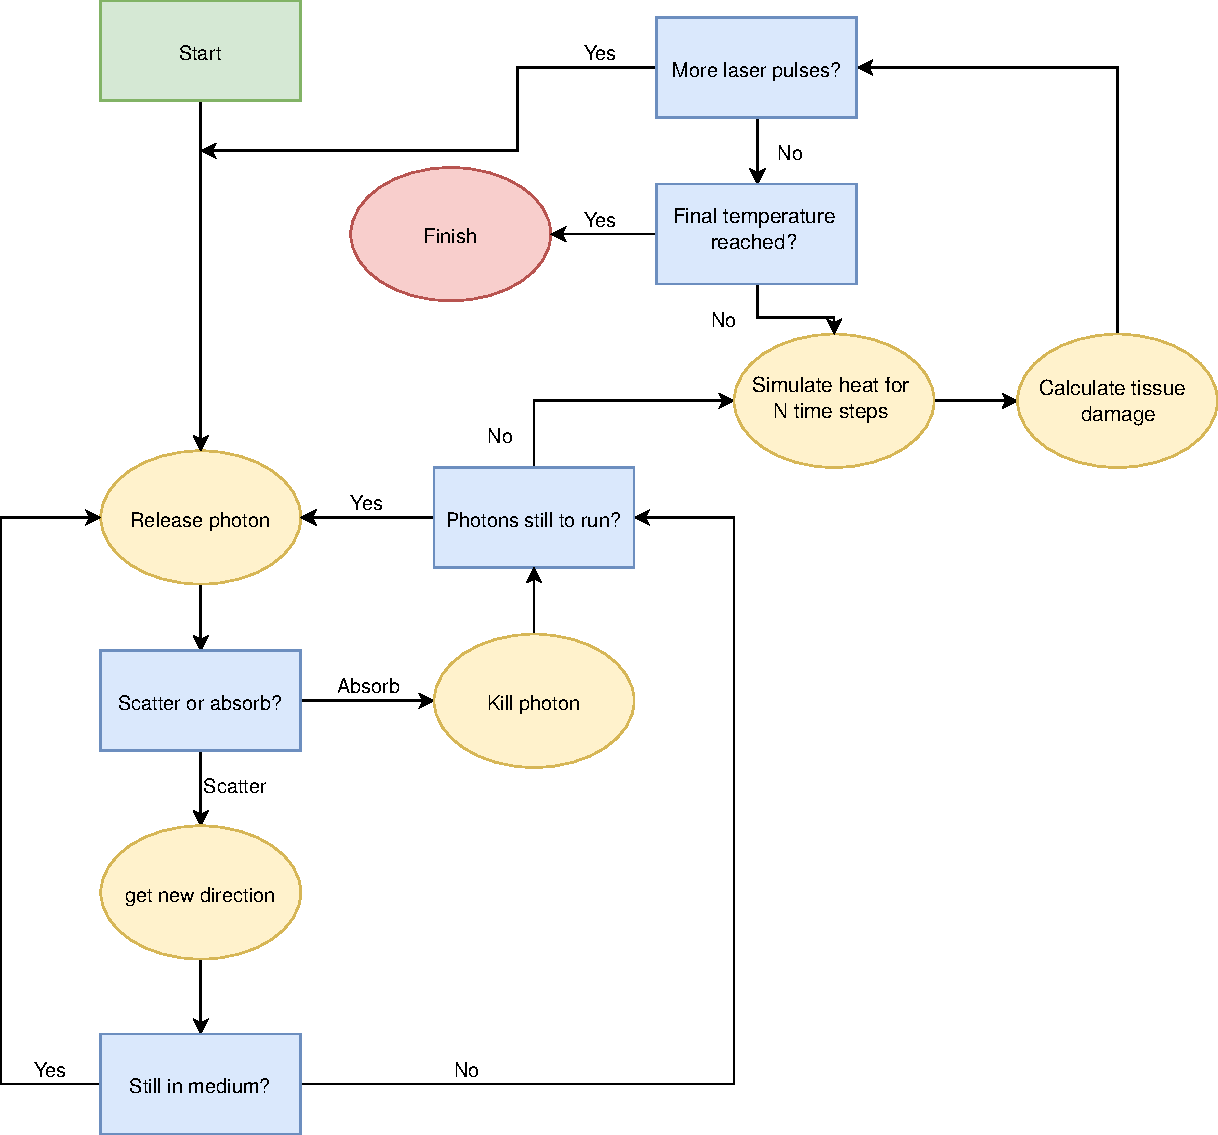
\includegraphics[scale=0.5]{./ablation/images/flowchart.pdf}
\caption{Flowchart of the tissue ablation algorithm.}
\label{fig:algo}
\end{figure}

To calculate the energy absorbed in the porcine tissue via the laser we use the path length counter method devised by Lucy \cite{lucy1999computing} (see~\cref{fig:jmea-explain}). The energy absorbed per voxel is therefore calculated as:

\begin{equation}
E_{i}^{abs} = \frac{L}{N \Delta V_i}\sum\mu_{a,i} s
\label{eqn:Eabs}
\end{equation}

\noindent Where:

	\indent L is luminosity [$W$];
	
	\indent N is the number of photons;
	
	\indent $\Delta V_i$ is the volume of the $i^{th}$ voxel [$m^{-3}$];
	
	\indent $\mu_{a,i}$ is the absorption coefficient of the $i^{th}$ voxel [$cm^{-1}$];
	
	\indent and s is the pathlength of a photon packet through the $i^{th}$ voxel [$cm$].
	
	\medskip
	
\begin{figure}
\centering
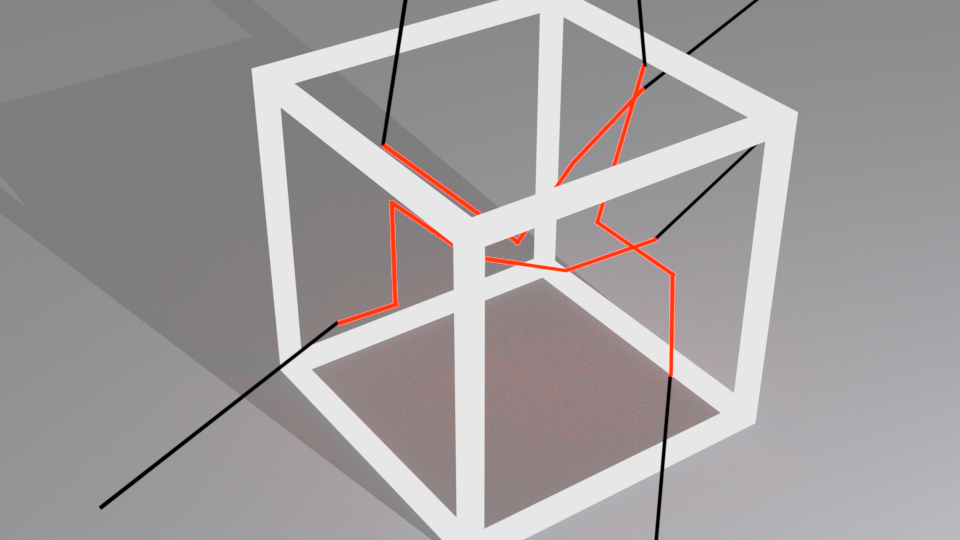
\includegraphics[scale=0.25]{./ablation/images/jmea-explain.png}
\caption{Red lines are photon paths within a voxel. Black lines photon paths out with the voxel. Red photon paths are summed up in order to calculate the absorbed energy within each voxel.}
\label{fig:jmea-explain}
\end{figure}	
		
This grid of absorbed energy is then passed to the heat transport portion of the simulation, so that the heat diffusion in the porcine tissue can be calculated.
\newpage
\subsection{Heat transport}

The diffusion of heat can be modelled using the heat equation~(\cref{eqn:heat}), which is derived from Fourier's law and the principle of conservation of energy~\cite{widder1976heat}~(see~\cref{app:heatderive}). 
The standard heat equation is a partial differential equation of the parabolic form. Solutions and analytical methods are readily available for lower dimensions (i.e. 1D heat diffusion), but for higher dimensions such as three dimensions, numerical models must be used for all bar the simplest problems.~The simplest form of the heat equation is shown below:

\begin{equation}
\rho c_p \frac{\partial T}{\partial t}= \nabla \cdot (\kappa \nabla T) + \dot{q}
\label{eqn:heat}
\end{equation}

\noindent Where:

	\indent $T(x, y, z, t)$ is the temperature as a function of time and space [\textit{K}];
	
	\indent $\kappa$ is the thermal conductivity [$W\cdot m^{-1}\cdot K^{-1}$];
	
	\indent $\rho$ is the density [$Kg \cdot m^{-3}$];
	
	\indent $c_p$ the specific heat capacity [$J\cdot K^{-1}$];
	
	\indent $\dot{q}(x,y,z,t)$ is the source/sink term as a function of time and space [$W\cdot m^{-3}$].
	
	\medskip

\Cref{eqn:heat} is for a homogeneous system where the thermal properties do not change as function of time, space and/or temperature. However in order to model a moving ablation front we must therefore use the non-linear heat equation where the thermal properties can be a function of time, space and/or temperature~(\cref{eqn:nonlinearheat}).

\begin{equation}
\frac{\partial T}{\partial t} = \frac{1}{(\rho c_p)_{\xi}}(\nabla k_\xi T + k_\xi\nabla^2T)+\dot{q}\quad \xi=(i,j,k)
\label{eqn:nonlinearheat}
\end{equation}

We have also included in the~\cref{eqn:nonlinearheat} a source and sink term to allow the modelling of heat loss/gain from external sources/sinks. The $\dot{q}$ term is a heat source/sink term. The heat source in this simulation is due to the laser, and we assume the only loss of heat to the surrounding medium is via convection and conduction.
	
These boundary conditions must be considered. All faces of the cube, bar the laser facing face, are considered to be pinned at 5$^{\circ}$C, as the porcine skin was kept cooled prior to experimental work and the simulation volume is smaller than the porcine tissue samples. The laser facing face has a simple convective BC:	

\begin{equation}
\dot{q}_c = -hA(T - T_\infty)
\label{eqn:bceqns}
\end{equation}

\noindent Where:

	\indent \textit{h} is the heat transfer coefficient [$W\cdot m^{-2}\cdot K$];
	
	\indent \textit{A} is the area of the grid element, that is radiating/convicting heat away [$m^{-2}$];
	
	\indent and $T$, and $T_\infty$ are the temperature in a voxel and the surrounding medium temperature respectively~[$K$].
	
	\medskip

As \cref{eqn:nonlinearheat} is generally hard to solve in arbitrary geometries with complex boundary conditions we employ a numerical method to solve \cref{eqn:nonlinearheat}.
The numerical method we employ is a \gls{fdm}. The \gls{fdm} is derived from the Taylor series approximation for derivatives. A function $f(x)$ is discretised onto a grid with \textit{N} nodes (see~\cref{fig:fdmexplain}). Then at a node \textit{i} we can use the Taylor series approximation in the forward ($+\text{ive}\ x$ direction) and backward ($-\text{ive}\ x$ direction) to give the derivatives in~\cref{eqn:fdmfwd,eqn:fdmbck}. Where: \textit{i} is the grid point at $x_o$, $i$+1 is the point at $x_0+\Delta x$, and \textit{i}-1 is the grid point at $x_{o}-\Delta x$. We can then combine these `forward' and `backward' derivatives to give a `central' derivative~\cref{eqn:fdmcent}. We can also give expressions for the $2^{nd}$ order derivatives for backward, forward and central (forward and backward $2^{nd}$ order equations omitted for brevity)~\cref{eqn:fdmcent2}.

\begin{figure}
  \begin{center}
    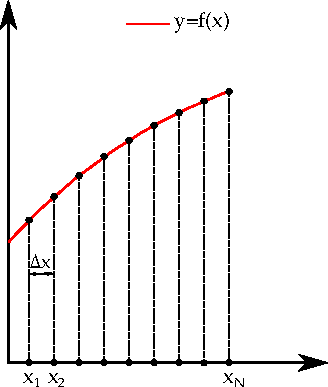
\includegraphics[width=0.48\textwidth]{./ablation/images/fdm.pdf}
  \end{center}
  \caption{Discretisation of \text{f(x).}}\label{fig:fdmexplain}

\end{figure}

\begin{subequations}
\begin{align}
\frac{df}{dx} &= \frac{f_{i+1} - f_{i}}{\Delta x}  &(forward) \label{eqn:fdmfwd}\\
\frac{df}{dx} &= \frac{f_{i} - f_{i-1}}{\Delta x}  &(backward) \label{eqn:fdmbck}\\
\frac{df}{dx} &= \frac{f_{i+1} - f_{i-1}}{2\Delta x}  &(central)\label{eqn:fdmcent}\\
\frac{d^2f}{dx^2} &= \frac{f_{i-1}-2f_i+f_{i+1}}{\Delta x^2} &(central)\label{eqn:fdmcent2}
\end{align}
\end{subequations}


Thus the linear heat equation~\cref{eqn:heat}, in 1D, taking a $1^{st}$ order forward time derivative, and a $2^{nd}$ order central spatial derivative gives:

\begin{subequations}
\begin{align}
\frac{T^{n+1}_i-T^{n}_i}{\Delta t} &= \alpha\frac{T^n_{i-1}-T^n_{i}+T^n_{i+1}}{\Delta x^2}  + \frac{\dot{q}}{\rho c_p}\\
T_{i}^{n+1} &=  \alpha\Delta t \frac{T_{i-1}^n-2T_i^n+T_{i+1}^n}{\Delta x^2} + \frac{\dot{q}}{\rho c_p}
\label{eqn:simplefdm}
\end{align}
\end{subequations}

\begin{figure}
  \begin{center}
    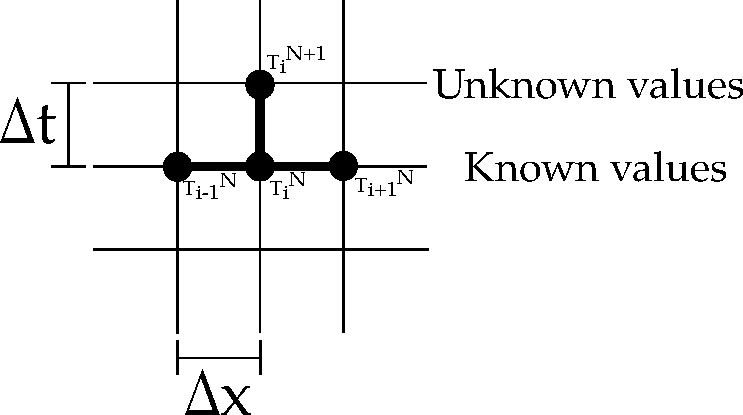
\includegraphics[width=0.48\textwidth]{./ablation/images/fdm-stencil.pdf}
  \end{center}
  \caption{Finite difference method stencil for simple explicit scheme}\label{fig:fdmstencil}
\end{figure}

\Cref{eqn:simplefdm} is called the `simple explicit form of finite-difference approximation'\cite{ozisik1994finite}. \Cref{fig:fdmstencil} shows the `stencil' of this scheme, where there are three known points at time \textit{N}, and just one unknown at time \textit{N+1}. There are various other scheme that can be used to calculate the temperature at the the next time step. However we use a simple explicit scheme here, due to its ease of implementation despite its stability being constrained in comparison to an implicit method. This method is also easily scaled up to 3D with little difficulty.

\medskip

For the more complicated non-linear heat equation we have to account for the possibility that the medium is not continuously smooth between nodes, in terms of optical and thermal properties. The two easiest methods~\cite{ozisik1994finite} of achieving this is: One, lag the value behind by one step, i.e $c_{p}^{n+1}=c_{p}^{n}$. Two, average $\kappa,\ \rho,\ \text{and}\ c_p$ using a half difference scheme where the thermal property used in the calculation is the thermal property half way between two nodes, i.e the average of the two nodes:

\begin{align}
\kappa^{\pm}&=\frac{\kappa_i+\kappa_{i\pm 1}}{2}\\
\rho^{\pm}&=\frac{\rho_i+\rho_{i\pm 1}}{2}\\
c_p^{\pm}&=\frac{c_{p,i}+c_{p,i\pm 1}}{2}
\end{align}

Thus for the simple 1D case as in~\cref{eqn:simplefdm}, we average the thermal properties when computing the coefficients of the temperature nodes, and lag the thermal properties when adding the heat from the laser:

\begin{equation}
T^{N+1}=\Delta t (AT^N_{i-1}-2BT^N_{i}+DT^N_{i+1})+ T_i^N + \frac{\dot{q_L}}{\rho c_p}\label{eqn:heatnonlin1d}
\end{equation}

Where:
\begin{align}
A=&\frac{\kappa^{-}}{\rho^{-}c_{p}^{-}2\Delta x^2} \nonumber \\
B=&\frac{\kappa^{+}}{\rho^{+}c_{p}^{+}2\Delta x^2} \label{eqn:coeffsABD}\\
D=&\frac{(A+B)}{2} \nonumber
\end{align}

\Cref{eqn:heatnonlin1d} can be generalised to higher dimensions easily. The 3D case gives:

\begin{align}
U_{xx} &=  (A T^N_{i-1,j,k} - 2B T^N_{i,j,k} + D T^N_{i+1,j,k}) \label{eqn:FDMheat1}\\
U_{yy} &=  (A T^N_{i,j-1,k} - 2B T^N_{i,j,k} + D T^N_{i,j+1,k}) \label{eqn:FDMheat2}\\
U_{zz} &=  (A T^N_{i,j,k-1} - 2B T^N_{i,j,k} + D T^N_{i,j,k+1}) \label{eqn:FDMheat3}\\
T^{N+1}_{i,j,k} &= \Delta t\ (U_{xx} + U_{yy} + U_{zz}) + T^{N}_{i,j,k} + \tfrac{\Delta t}{\rho c_p}\dot{q_L} \label{eqn:FDMheat4}
\end{align}

\noindent Where:

	\indent $T^{N+1}_{i,j,k}$ is the new temperature at node $i,j,k$ [$K$];
	
	\indent $T^N_{i,j,k}$ is the temperature at node $i,j,k$ at the current time step [$K$];
	
	\indent $\alpha$ is the thermal diffusivity [$m^2\cdot s^{-1}$];
	
	\indent $\kappa$ is the thermal conductivity [$W/m\cdot K$];
	
	\indent $\Delta x\ etc.$ is the size of the grid element in the $p^{th}$ direction [$m$];
	
	\indent and $A, B,D$ are the coefficients in their respective dimension (\cref{eqn:coeffsABD}).

	\medskip
	
Incorporating B.Cs on the top air exposed face:

\begin{equation}
U_{zz} = \tfrac{\alpha}{\Delta z^2} (\tfrac{2 \Delta z}{\kappa} (-h(T^N_{i,j,k}-T^N_\infty) ) -2 T^N_{i,j,k} + 2T^N_{i,j,k+1})\label{eqn:bceqn} 
\end{equation}

\Cref{eqn:FDMheat4,eqn:bceqn} give the full numerical solution to the non-linear heat equation with a convection boundary term and laser heat source. This will allow us to calculate the heat diffusion in the porcine tissue due to laser heating.

\medskip

As the laser used in the experimental work, operates in a pulsed mode, we account for this in our simulation. We assume that the pulse shape is a top-hat pulse. In the heat simulation we have an additional variable in the term $laserOn\cdot\tfrac{\alpha \Delta t}{\kappa}\dot{q_L}$ in \cref{eqn:FDMheat4}. This additional variable, $laserOn$, is a boolean value, which is defined as:

\[   
laserOn = 
     \begin{cases}
       \text{1,} &\quad\text{Laser on}\\
       \text{0,} &\quad\text{Laser off}.\\
     \end{cases}
\]

In the instance where there is more than one pulse, the laser is turned on and off based upon the pulse frequency.

\medskip

As we are using a simple explicit \gls{fdm}, the time step is constrained in order to make the solution stable. For a cubic 3D \gls{fdm} without prescribed flux BCs, yields the constraint: $\Delta t \leq \tfrac{1}{\delta \alpha}$ where $\delta=\tfrac{1}{\Delta x^2}+\tfrac{1}{\Delta y^2}+\tfrac{1}{\Delta z^2}$. However as we have a convection prescribed boundary condition, the constraint on the time is more severe. Along with this time restraint, the pulse length of the laser also has to be considered. If the time step of the heat simulation is too large it will not account for the heat deposited by the laser. Thus, the timestep has to be an order of magnitude smaller than the shortest laser pulse.

As the timestep is small, and the grid resolution large, the resultant simulation is slow. Thus the code has been fully parallelised to improve performance. Both the \gls{mcrt} and heat simulation are independently parallelised. As discussed in~\cref{chap:mcrt}, the \gls{mcrt} simulation is fully parallelised, and the results are passed to the heat simulation.

\medskip

Parallelisation of the heat simulation is more involved than the `embarrassingly parallel' class of problems that \gls{mcrt} belongs to. This is due to the heat simulation being dependant on the temperature of adjacent nodes. Thus information will have to be passed from each individual core during computation, as opposed to doing the information passing at the end of the simulation \textit{\`a la} \gls{mcrt} parallelisation.
The heat simulation is parallelised using a technique called `halo swapping'. This involves splitting up the computational domain (see \cref{fig:griddecomp}), in this case the tissue medium, and doing the calculations on each domain on a separate core. The `halo swapping' comes in when cores need to communicate with each other about updating their boundary temperature nodes (see \cref{fig:haloswap}).

* old data from before nonlinear heat equation *
On a workstation computer these simulations were carried out on (Intel Xeon E3-1245 v5, 8 core @ 3.5GHz) led to a speed up of $\sim$6, over the serial simulation. Using Amdahl's law\cite{amdahl1967validity}, the serial portion of the simulation is $\sim$ 5\%, giving a theoretical speed up $\sim$ 20 times the serial simulation.


\begin{figure}
\vspace{-45pt}
\centering
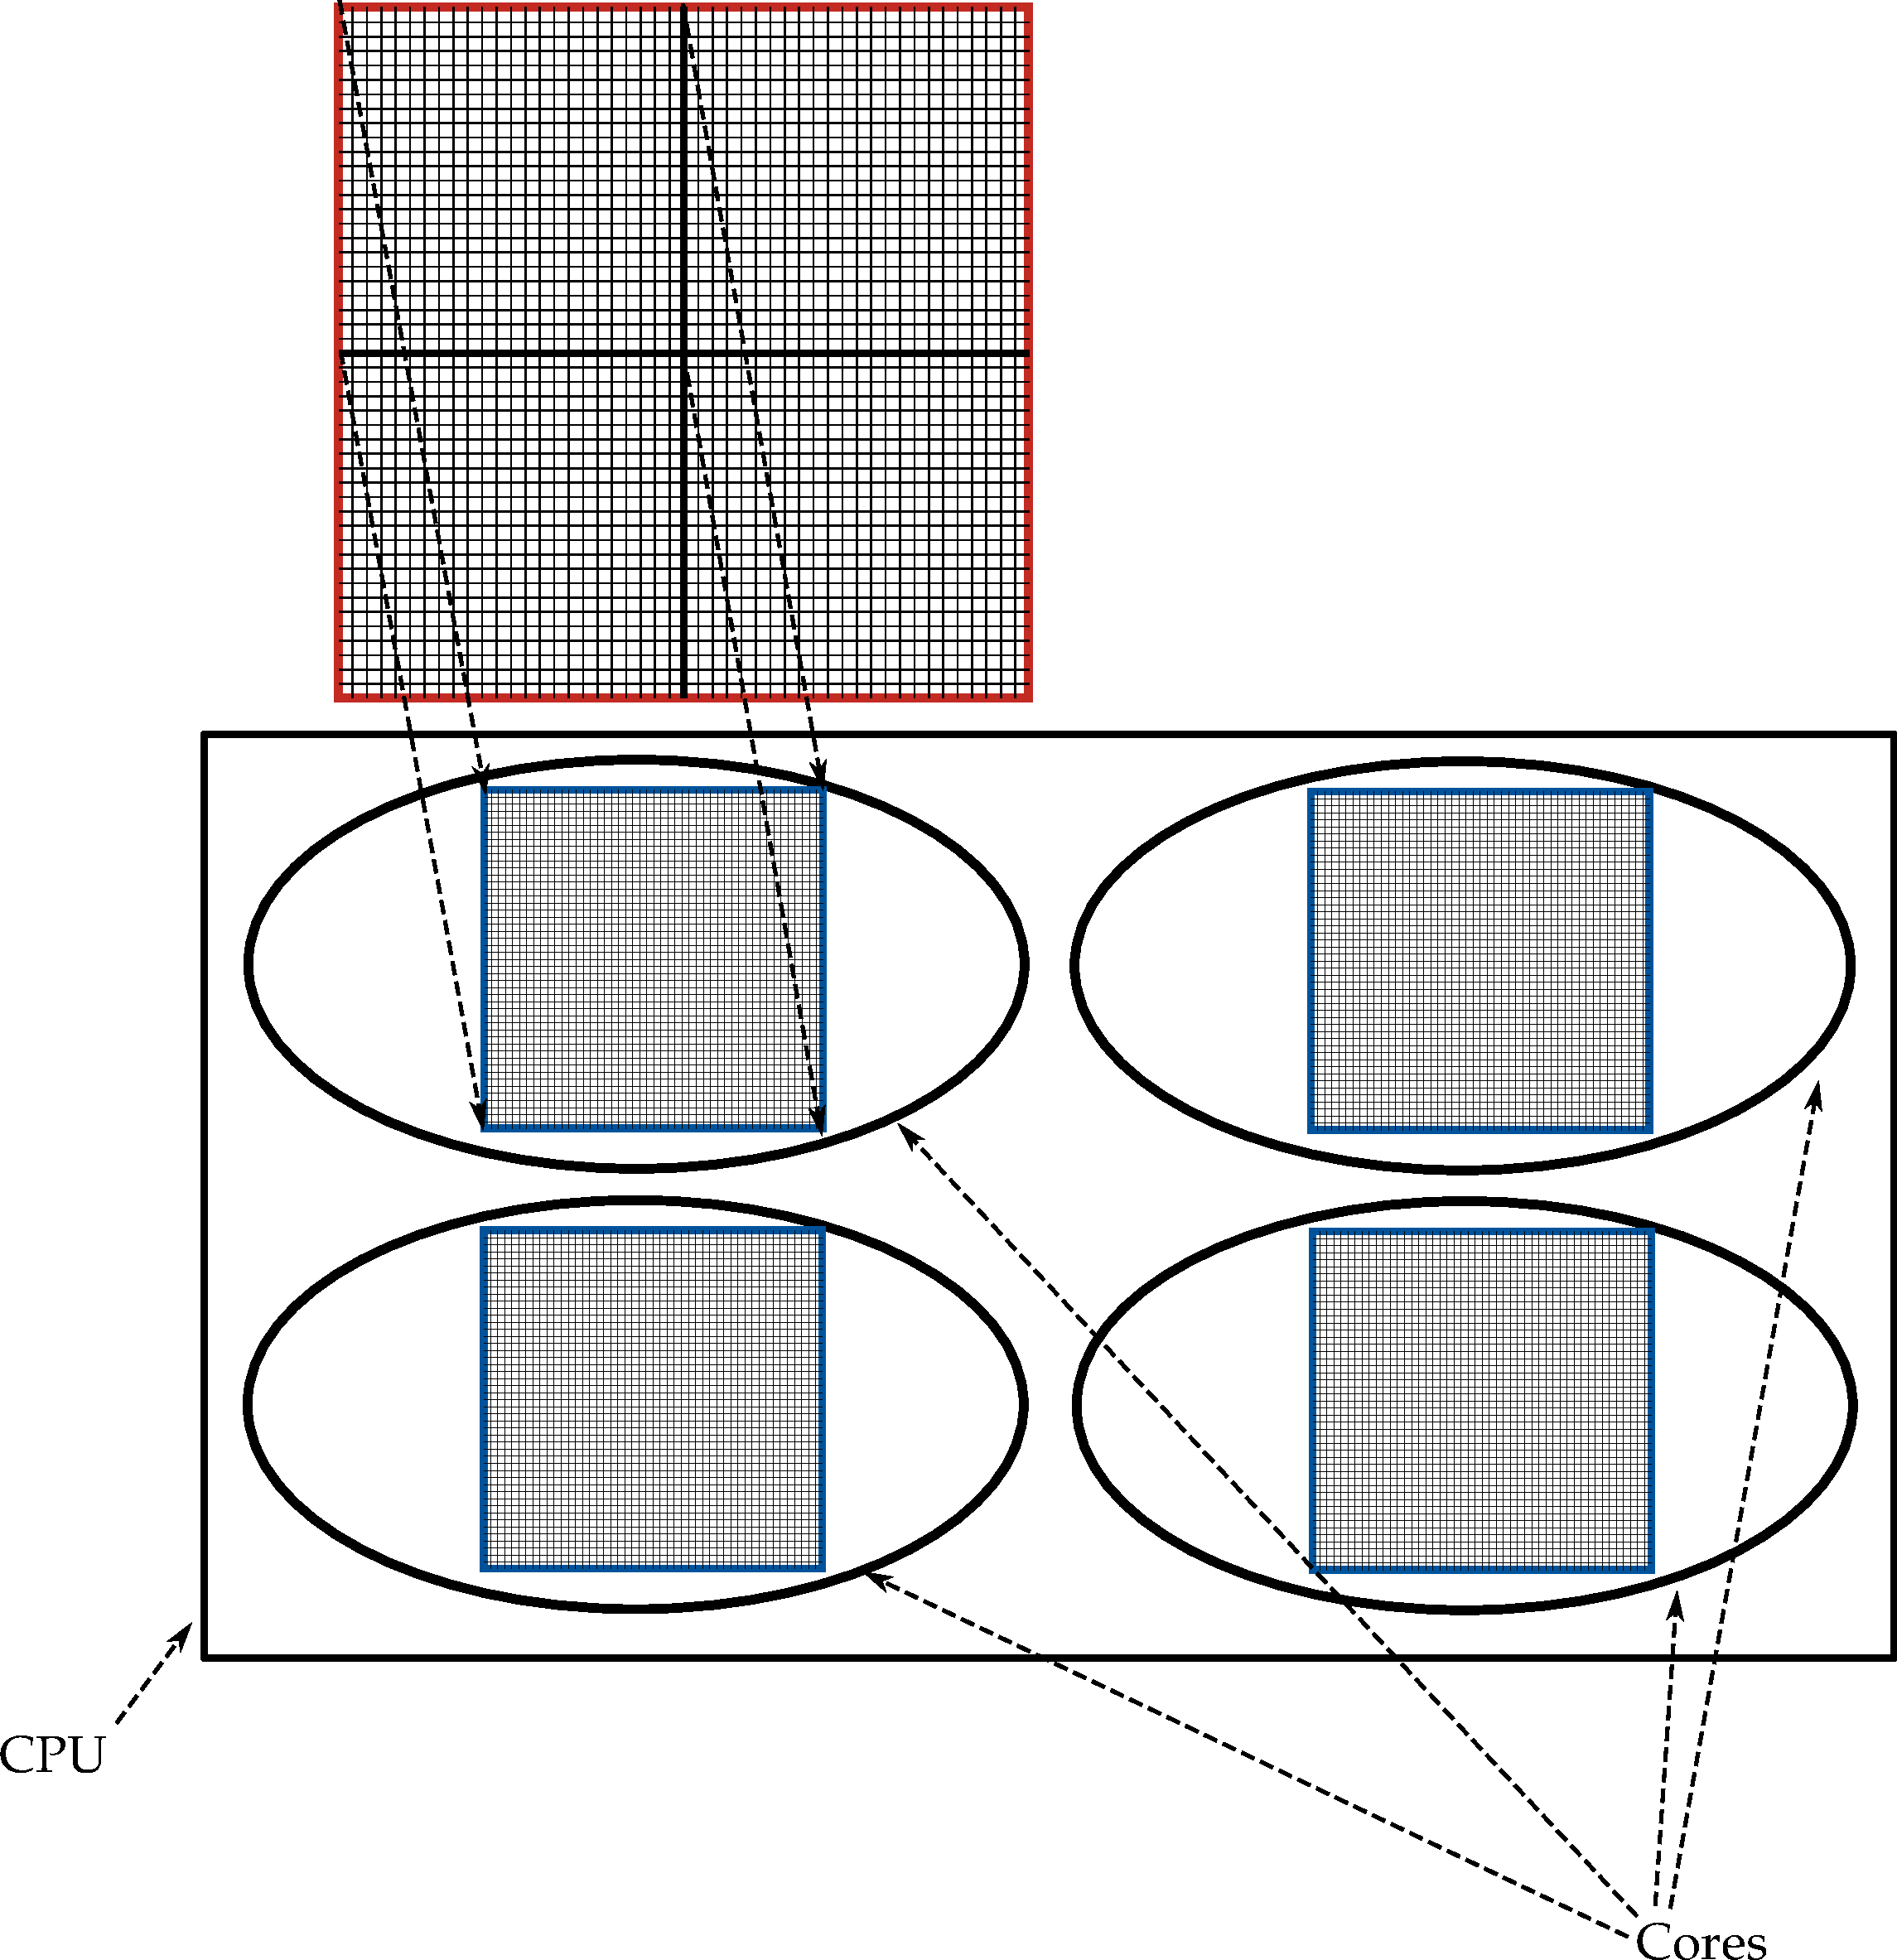
\includegraphics[scale=.35]{./ablation/images/grid-decomp.pdf}
\caption{Computational domain decomposition. Total computational domain (red outline) is evenly divided between cores in the CPU. This is done via layers of the domain in the z direction. Information is passed to/from cores via the `halo swap' process (see~\cref{fig:haloswap}).}
\label{fig:griddecomp}
\vspace{-10pt}
\end{figure}

\begin{figure}
\centering
\def\svgwidth{350pt}
\input{./ablation/images/halo.pdf_tex}
\caption{Halo swapping. Process A updates the area in red and blue on the left. It updates the blue area which is sent to process B as B's `halo'. Process B cannot update it's own halo, but rather updates the halo for process A.}
\label{fig:haloswap}
\end{figure}


After one time step of the heat simulation has been completed, the temperature grid is passed to the tissue damage portion of the simulation to calculate the tissue damaged that may have accrued during the heat simulation timestep.

\subsection{Tissue Damage}
\label{sec:tissuedamage}

\subsubsection{Introduction}
The final portion of the simulation is the tissue damage model. To be able to model damage to the tissue we first need to be able to describe the tissue damage process due to heating from a laser.

When the laser is turned on, the temperature starts to rise within the tissue due to the absorption of photons by the tissue. The temperature rise causes damage to the tissue when above a threshold temperature, $T_d$, approximately 43$^{\circ}C$~\cite{welch2011optical}*p539*. From the temperature, $T_d$, we define four main areas of tissue damage:


\begin{equation}
T = 
     \begin{cases}
       \text{coagulation,} &\quad T_d\leq T \leq 100~^{\circ}C\\
       \text{water boils,} &\quad T=100~^{\circ}C\\
       \text{carbonisation,} &\quad 100~^{\circ}C \leq T \leq T_a\\
       \text{ablation,} &\quad T=T_a.\\
     \end{cases}
\end{equation}


The area of tissue damage we term `coagulation' is a multifaceted process. At 43$^{\circ}$C - 50$^{\circ}$C, bonds break within cell membranes, causing ruptures, and some cell death~\cite{welch2011optical,wright2015quantitative}. This process is usually termed \textit{hyperthermia}. Around 50$^{\circ}$C, enzyme activity decreases, cells become immobile, and various cell repair mechanisms are disabled, leading to increased cell death. When temperatures exceed 60$^{\circ}$C, proteins become denatured. Thermal denaturation is a structural and functional change in a protein due to the heating it undergoes. This means they change from a highly organised structure with specific purposes, to disorganised structures with little to no function at all.  A classic example of denaturation of proteins, is in cooking eggs. Denaturation occurs when the clear fluid egg white, rich in protein albumin, becomes a solid white~\cite{niemz2013laser}.

The next stage in the tissue damage process is the vaporisation of water. As the temperature of the tissue starts to approach 100${^{\circ}}$C (at 1 atm), water starts to vaporise. If the vaporised water cannot escape the tissue it forms steam vacuoles, small pockets of steam. These vacuoles can easily been seen when viewing tissue samples after tissue has been treated with a high powered laser (see \cref{fig:histology}). In certain conditions these steam pockets can explode, with these `explosions' being audible by the human ear~\cite{petrella2013popcorn}.


The third stage of tissue damage is carbonisation or caramelisation of the tissue. This occurs when most of the water has boiled off, leaving the remaining tissue to heat up and reduce to its elemental carbon form. This carbonisation of tissue, when it occurs, is generally only a thin layer of 5-20~$\mu m$~\cite{welch2011optical,verdaasdonk1990explosive}.

The final stage of tissue damage is the removal of the remaining tissue, i.e tissue ablation. There is no agreement in the literature how tissue undergoes ablation with a number of methods proposed~\cite{vogel2003mechanisms,mckenzie1990physics}. The tissue ablation process is not a simple process, with various unknowns which depend on everything from tissue composition to laser power, wavelength, and pulse length. The literature however, does suggest that it takes place when the tissue temperature is between 177 and 500${^{\circ}}$C\cite{gerstmann1994char,mckenzie1986three,sagi1992heating}.

\begin{figure}	
\vspace{-10pt}
	\centering
	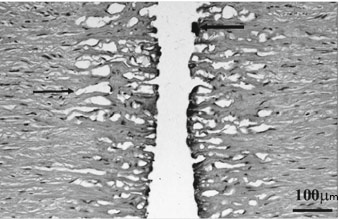
\includegraphics[width=\columnwidth]{./ablation/images/steam_vacoule.png}
	\caption{Tissue ablations, as viewed under a microscope. Steam vacuoles are clearly visible either side of the ablation area. Carbonisation is also evident at the edges of the ablation fronts. Adapted from~\cite{welch2011optical}.}
	\label{fig:histology}
	\vspace{-10pt}
\end{figure}

In order to model all these tissue damage processes we split our tissue damage model into two sections: `physical' damage and coagulation damage. Where `physical' damage changes the tissue optical and thermal properties, where the coagulation damage has no effect on the tissue's bulk optical or thermal properties.

\subsubsection{Modelling coagulation damage}\label{sec:coagdamage}
With the description of the various process that tissue undergoes during ablation, we can now create a numerical model of these processes.
First, in order to model the full extent of the damage done under 100${^{\circ}}$C, i.e in the coagulation regime, we use the Arrhenius damage model. The Arrhenius damage model was originally used as a kinetic model of reaction products in chemistry~\cite{pearce2009relationship}. It has since been adapted by various authors for modelling tissue damage, and is the \textit{de facto} standard \cite{hendriques1947studies,jiang2002effects}. These authors and various others, adapted this model by fitting \cref{eqn:arrhenius} to experimental data for burn damage. The two parameters fitted are A, the frequency factor, and $\Delta E$, the activation energy.

\begin{equation}
\Omega(t)=\int^{t_{f}}_{t_i} Ae^{(-\tfrac{\Delta E}{RT})}d\tau
\label{eqn:arrhenius}
\end{equation}


\noindent Where:

	\indent $\Omega$ is the damage value;
	
	\indent A is `frequency factor' [$s^{-1}$];
	
	\indent $\Delta E$ is activation energy [$J\cdot mol^{-1}$];
	
	\indent R is the universal gas constant [$J\cdot mol^{-1}\cdot K^{-1}$];
	
	\indent T is the temperature [$K$];
	
	\indent and $t_i$ and $t_f$ are the initial time and final time at $t_{crit}$.
	
	\medskip

It is reported that a value of $\Omega$ of 0.53, 1.0, and 10$^4$ relate to first, second, and third degree burns respectively~\cite{diller1983finite}. We use the Arrhenius damage model in order to better understand the amount of damage caused by the laser in the non-ablated areas of tissue.

\subsubsection{Modelling physical tissue damage}

As tissue mostly consists of water~\cite{meglinski2002quantitative} when the temperature of the tissue approaches 100$^{\circ}$C (at 1 atm), water in the tissue begins to boil off. This acts as a large heat sink for the absorbed laser energy, slowing down the rate of ablation. The energy required to boil the water is $Q_{vapor}=m_v\cdot L$, where $m_v$ is the mass of a voxel, and $L$ is the latent heat of vaporisation. The energy to boil off the water is provided via the laser and heat diffusing into the voxel:

\begin{equation}
Q_{vapor}=\underbrace{laserOn\cdot\dot{q}\cdot \Delta t\cdot V_{i,j,k}}_\text{laser heating} + \underbrace{c\cdot M_{i,j,k}\cdot\Delta T}_\text{heat diffusion}
\end{equation}

\noindent Where:

	\indent $Q_{vapor}$ is the current energy in Joules that has been used to boil off the water in the voxel [$J$];
	
	\indent $laserOn$ is a boolean variable that determine if the laser is on or off [$-$];
	
	\indent $\dot{q}$ is the energy absorbed by the voxel due to the laser [$W\cdot m^{-3}$];
	
	\indent $\Delta t$ is the timestep [$s$];
	
	\indent $V_{i,j,k}$ is the volume of the $i^{th}$, $j^{th}$, $k^{th}$ voxel [$m^3$];
	
	\indent $c$ is the heat capacity of the voxel [$J\cdot K^{-1}$];
	
	\indent $M_{i,j,k}$ is the mass of the $i^{th}$, $j^{th}$, $k^{th}$ voxel [$Kg$];
	
	\indent and $\Delta T$ is the change in temperature the voxel would undergo, if the water was not boiling off.

	\medskip
	
As water boils off, the water content of each voxel changes. This affects the absorption coefficient, density, thermal conductivity, and heat capacity. Each of these vary with water content per voxel\cite{choi2001analysis};

\begin{align}
W &= W_{init} - \left(W_{init} \cdot \left(\tfrac{Q_{current}}{Q_{vaporisation}}\right)\right) \\
\rho &= \frac{1000}{W + 0.649\cdot P} \\
c_p &= 4.2\cdot 10^{3}\cdot W + 1.09\cdot 10^{3}\cdot P \\
\kappa &= \rho \cdot (6.28\cdot 10^{-4}\cdot W + 1.17\cdot 10^{-4} \cdot P)\\
\mu_a &= W \cdot \mu_{water} + \mu_{protein}\\
\end{align}

\noindent Where:

\indent $W$ is the water content (i.e W = 0.7 equates to 70\% water content);

\indent $W_{init}$ is the initial water content;

\indent $Q_{current}$ is the total energy absorbed by the $i^{th}$ voxel since the temperature reached 100$^{\circ}$C [$J$];

\indent $P$ is the protein content (i.e P = 1.0 - W);

\indent $\kappa$ is the Thermal conductivity [$W\cdot m^{-1}\cdot K^{-1}$];

\indent $c_p$ is the heat capacity [$J\cdot Kg^{-1}\cdot K^{-1}$];

\indent and $\mu_a$ is the total absorption coefficient, and $\mu_{water}\ \text{and}\ \mu_{protein}$ are the absorption coefficients of water and protein respectively.

\medskip

We define the \gls{ta} as occurring between 177 and 500$^{\circ}$C\cite{gerstmann1994char,mckenzie1986three,sagi1992heating}. At \gls{ta} the tissue is removed and the thermal, optical, and physical properties set to that of air.

The updated damaged tissue structure is then fed back to the \gls{mcrt} model and the whole process repeats until the predefined time limit is reached. This whole process of photon propagation, heat diffusion and tissue damage is outlined in \cref{fig:algo}.

\subsection{Validation}

\subsubsection{Heat transport validation}

In order to thoroughly validate the numerical method we employ to solve the heat equation, we compare the numerical method against an easily solvable analytical case. We solve the heat equation on a cube, side L, in a surrounding medium of 0$^{\circ}$C. The cube is initially at temperature 37$^{\circ}$C and we calculate the temperature at time \textit{t=0.1s}. Thus the boundary conditions are:

\begin{align}
T(0,y,z,t)&=T(x,0,z,t)=T(x,y,0,t)=0^{\circ}\text{C} \label{eqn:bc1}\\
T(L,y,z,t)&=T(x,L,z,t)=T(x,y,L,t)=0^{\circ}\text{C} \label{eqn:bc2}
\end{align}

The thermal diffusivity~($\alpha$), density~($\rho$), and heat capacity~($c_p$) are all set to 1. Assuming a separable solution in Cartesian coordinates yields:

\begin{equation}
\begin{split}
T(x,y,z,t)=&(A_1 cos(\alpha x) + A_1 sin(\alpha x))\cdot\\
&(B_1 cos(\beta y) + B_1 sin(\beta y))\cdot\\
&(C_1 cos(\gamma z) + C_1 sin(\gamma z))\cdot e^{-\alpha\mu^2t}\\
\end{split} 
\end{equation}

\begin{equation}
\mu^2=\alpha^2+\beta^2+\gamma^2
\end{equation}

Applying the boundary conditions (\cref{eqn:bc1,eqn:bc2}) gives:

\begin{equation}
A_1=B_1=C_1=0\
\text{and}\ \alpha=\frac{\pi n}{L}\ \beta=\frac{\pi m}{L}\ \gamma=\frac{\pi p}{L}
\end{equation}

\begin{equation}
\therefore  T_{nmp}(x,y,z,t)=A_{nmp}\cdot sin\left(\frac{\pi n x}{L}\right)\cdot sin\left(\frac{\pi m y}{L}\right)\cdot sin\left(\frac{\pi p z}{L}\right)
\end{equation}

This yields the following solution for the heat equation using the principle of superposition, and solving \cref{eqn:heatfactoranalytic} with $f(x,y,z)$ as the initial temperature profile of the cube:

\begin{equation}
A_{nmp}=\frac{8}{L^3}\int_0^L\int_0^L\int_0^L f(x,y,z)\cdot sin(\frac{\pi n x}{L})\cdot sin(\frac{\pi n y}{L})\cdot sin(\frac{\pi n z}{L})\ dx\cdot dy\cdot dz
\label{eqn:heatfactoranalytic}
\end{equation}

\begin{equation}
T(x,y,z,t)=\sum^\infty_{n=1,3,..}\sum^\infty_{m=1,3,..}\sum^\infty_{p=1,3,..}\frac{2368}{\pi^3nmp}\cdot sin(\frac{\pi n x}{L})\cdot sin(\frac{\pi m y}{L})\cdot sin(\frac{\pi p z}{L})\cdot e^{(-\lambda^2t)}
\end{equation}

\noindent Where:

	\indent $\lambda^2=\alpha\pi^2(\tfrac{n^2}{L^2}+\tfrac{m^2}{L^2}+\tfrac{p^2}{L^2})$;
	
	\indent $n,m,p$ are odd integers;
	
	\indent and $L$ is the length of the cube.
	
	\medskip
	
At time, $t=0.1$s, a slice through the middle of the cube, $L=1~cm$,  yields \cref{fig:validation-heat}, which shows that the numerical method matches the analytical solution closely.

\begin{figure}	
\vspace{-10pt}
	\centering
	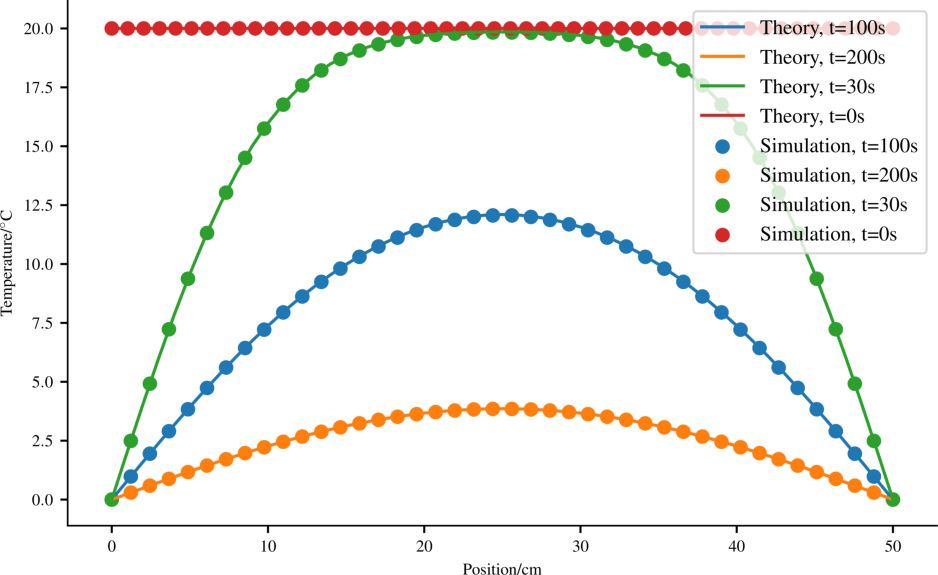
\includegraphics[width=\columnwidth]{./ablation/images/validation.pdf}
	\caption{Comparison between analytical solution and numerical method at t=0.1~$s$.}
	\label{fig:validation-heat}
	\vspace{-10pt}
\end{figure}	

\subsubsection{MCRT $\&$ heat transport validation}

As a first test of our code, both \gls{mcrt} and heat simulation, we compare to a simple analytical model of ablation. The simple model of ablation is as: We define the ablation energy ($E_a$) as the minimum energy required to raise the temperature of the medium to 100~$^{\circ}$C, and then boil off the water in a volume dV, mass M. Thus in one dimension we have~\cref{eqn:ablationenergy}, where the symbols have their usual meanings. If the energy for ablation is delivered in a time \textit{dt} by a laser of power density ($Wcm^{-2}$) this gives \cref{eqn:midequationablation}.~\Cref{eqn:midequationablation} can be rearranged in order to give an ablation front velocity, \cref{eqn:ablationvelo}.


\begin{align}
E_a &= c_p \rho dx \Delta T + L_v \rho dx \label{eqn:ablationenergy}\\
P\cdot dt &= \rho dx (c_p \Delta T + L_v) \label{eqn:midequationablation} \\
u &= \frac{P}{\rho(c_p\Delta T+ L_v)} \label{eqn:ablationvelo}
\end{align}

Assuming the ablation front moves with constant velocity during the ablation, and using $L_v=2.53\cdot 10^6\ J\cdot Kg^{-1},\ c_p=4181\ J\cdot Kg^{-1}\cdot K^{-1}$ and the medium is a cube side $2\ mm$, with a starting temperature is 37~$^{\circ}$C with a water content of 70\% giving a density of 700~$Kg\cdot m^{-3}$. For these parameters this gives an ablation velocity, $u\simeq 0.77\ cm\cdot s^{-1}$, and a time to ablate through 2~$mm$ of tissue of $\simeq 0.26~s$.
As the code developed in this chapter simulates the diffusion of heat in a medium due to an incident laser, the expected time to ablate through the same medium should be slightly less as heat diffuses away from the voxel while it is heated being heated. When the full heat + \gls{mcrt} code is used to simulate this experiment, it gives a time, $t \simeq 0.33~s$.	

\medskip

***maybe more? Could compare to https://doi.org/10.1117/1.2204615. They use MCRT + FDM but no ablation. So would be good test. Leaving till 2019 if time***


\section{\textit{In silco} results} 

\subsection{Introduction}

In order to match the experimental results, we must first create as accurate model of the experimental setup \textit{in silico}. However due to computational constraints, such as memory and time available, we must make some approximations to the experimental setup. The porcine skin was a large thin slice of the top most layers of the skin. However as the area of interest is where the ablation occurs, we initially  model the porcine skin as a cuboid, dimensions:  1.1 $\times$ 1.1 $\times$ 0.5 cm. The initial temperature of the porcine skin is assumed to be around 5$^{\circ}$, as the tissue was kept on ice or was kept cooled. 
As mentioned in the previous sections, there are several unknowns in the model: \gls{ta}, water content, temperature of air after ablation, and the exact thermal and optical properties of the porcine tissue. Therefore we run several models so that the full parameter space of these unknowns can be explored.
Results from these \textit{in silico} experiments are presented in this section along with a comparison of the model to the experimental work carried out in collaboration with the University of Dundee and the Photobiology department at Ninewells hospital.


\subsubsection{Optical \& thermal properties}

As mentioned, the thermal and optical properties of porcine tissue are not known exactly for a given tissue sample. This is due to no one tissue sample being exactly the same as another sample, due to various biological factors. As such the thermal and optical properties used in this section are taken from various literature sources.

The laser used in the experimental work is an infrared laser. This means that the optical properties of the tissue are dominated by water absorption (see \cref{fig:waterabsor}). The laser used in the experiment is the Pixel CO$_2$\cite{pixelco2}. The Pixel CO$_2$ laser has a wavelength 10.6$~\mu m$ which corresponds to an absorption of coefficient of $\sim 850~cm^{-1}$. As the absorption coefficient is large, we assume that scattering is negligent at these wavelengths.
\Cref{table:values} summarises the thermal properties for tissue and air used in the simulations.  

\begin{figure}	
%\vspace{-10pt}
	\centering
	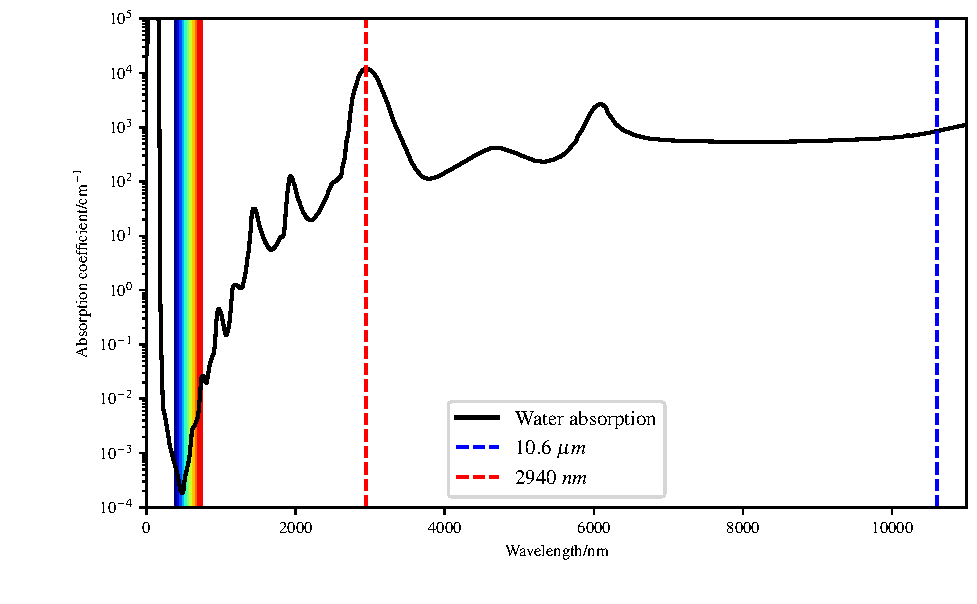
\includegraphics[width=\columnwidth]{./ablation/images/water.pdf}
	\caption{Water absorption coefficient for wavelengths 0-12000nm \cite{segelstein1981complex}. Data shows that water is highly absorbing in the infra-red portion of the spectrum  compared to the visible portion.}
	\label{fig:waterabsor}
	%\vspace{-10pt}
\end{figure}

\begin{table}
\begin{tabular}{|c|c|c|c|}
\hline 
• & Thermal conductivity, $\kappa$  & Density, $\rho$ & Heat capacity, c \\ 
\hline 
Tissue & $\rho \cdot (6.28\cdot 10^{-4}\cdot W + 1.17\cdot 10^{-4} \cdot P)$ & $\frac{1000}{W + 0.649\cdot P}$ & $4.2\cdot 10^{3}\cdot W + 1.09\cdot 10^{3}\cdot P$  \\ 
\hline 
Air & $a e^{-b(T-273.15)} +c$  & $\tfrac{p_{atm}}{R_{spec} T}$ & 1006 \\ 
\hline 
\end{tabular}
\caption{Optical and thermal properties for porcine tissue and air.}\label{table:values}
\end{table}  

The laser was used in `Pixel beam' mode. This means that the laser beam is split into an array of smaller beams. The laser used an array $9 \times 9$ of 81 pixel beams. The Pixel CO$_2$ laser was upgraded during the period in which the experimental data was taken, we present both sets of data, pre-upgrade and post-upgrade. The upgrade consisted of an update to the laser power, from $\sim$ 30~$W$ to $\sim$ 70~$W$.

The laser delivered one single pulse of varying energy over the range 50~$mJ$ to 400~$mJ$, in so called ``super pulsed mode". The experiment consisted of ablating the porcine tissue, as a function of energy per `pixel' beam. This was achieved by adjusting the pulse length of the laser, so that the energy per pulse was varied over a range 50~$mJ$ to 400~$mJ$. The energy range for the laser was kept the same pre and post-upgrade, with the pulse length differing.

\subsubsection{Computational speed up:}
As mentioned in the introduction, the volume of interest is the are around the ablation craters. The volume is 1.1 $\times$ 1.1 $\times$ 0.5~$cm$. However, in order for the simulation to have good resolution of the ablation craters, this volume would require a large number of voxels for the tissue model. This is infeasible due to: the memory required to store the various counters, grids, and variables, and the time that would be required in order to carry out the computation. Thus the volume of interest is reduced to focus on just one of the ablation craters that is created by the laser.
As a sanity check to ensure that we are not omitting any phenomena by focusing on just one ablation crater, an initial simulation that simulates the full volume of interest was carried out to investigate the possibility of overlapping craters or other related phenomena. The simulation, as shown in~\cref{fig:sizecheck}, gives us validation that the shrinking of the volume of interest is a valid approximation to make.

\begin{figure}
	\centering
    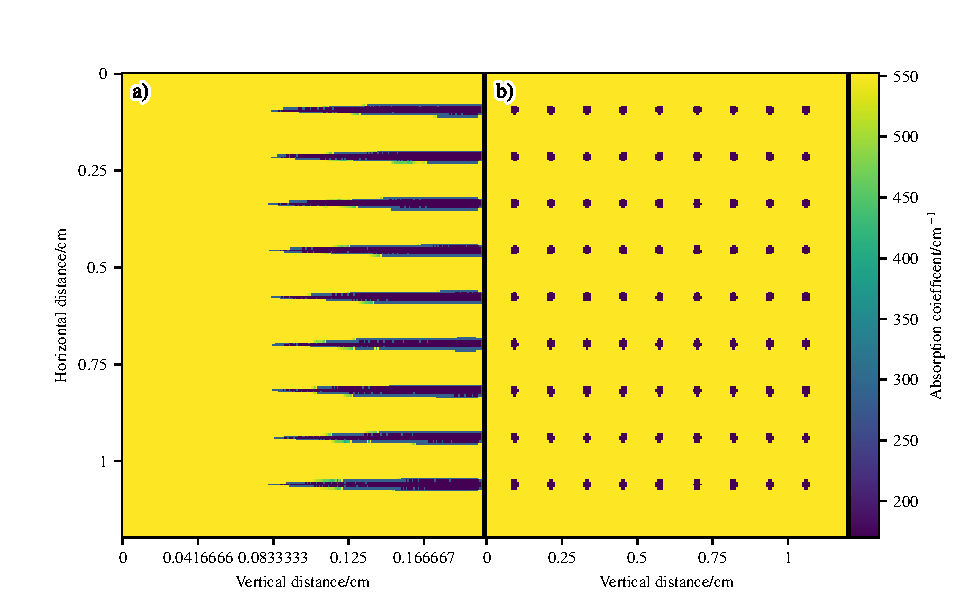
\includegraphics[width=\columnwidth]{./ablation/images/slice.pdf}
    \caption{Simulation of 81 pixel beams. Figure is a slice through the optical properties at the end of the simulation. Yellow is unchanged tissue, and purple is completly ablated tissue. Figure shows that the ablation craters do not overlap one another.}\label{fig:sizecheck}
\end{figure}

\subsection{Results}

\subsubsection{Investigating ablation temperature, \texorpdfstring{$T_a$}{Ta}}

Various literature sources report the ablation temperature ranging from 177$^{\circ}$ to 500$^{\circ}$~\cite{gerstmann1994char,mckenzie1986three,sagi1992heating}. Thus, we run several models over this range in order to establish a `good' \gls{ta} which fits with the experimental results. \Cref{fig:ta} shows how \gls{ta} affects the crater depth as a function of pixel beam energy for the CO$_2$ laser. Both *hopefully still awaiting data...* the 70~$W$ and 30~$W$ simulations agree, that a `good' \gls{ta} is around $T_a=400~^{\circ}C$.

Increasing the ablation temperature, has the obvious affect of requiring more energy to be deposited by the laser before ablation takes place. As more energy is required to heat the porcine tissue up to the ablation temperature before it can be ablated. This also allows more heat to diffuse away from the ablation crater increasing the thermal damage done to the surrounding tissue. Decreasing the ablation temperature has the converse affect, and allows the ablation crater to become deeper.

Over the full range of \gls{ta}, as the energy per pixel beam increases, there is a trend that at higher energies the crater depth tapers off. This is most likely due to a number of reasons. As the ablation craters grows the volume of tissue that is ablated is replaced with air, allowing more heat loss from the tissue to the environment. As well as heat loss to the environment, more heat is diffused away into the surrounding tissue as the crater grows, due to the availability of more tissue for the heat to diffuse into.


\begin{figure}
	\centering
    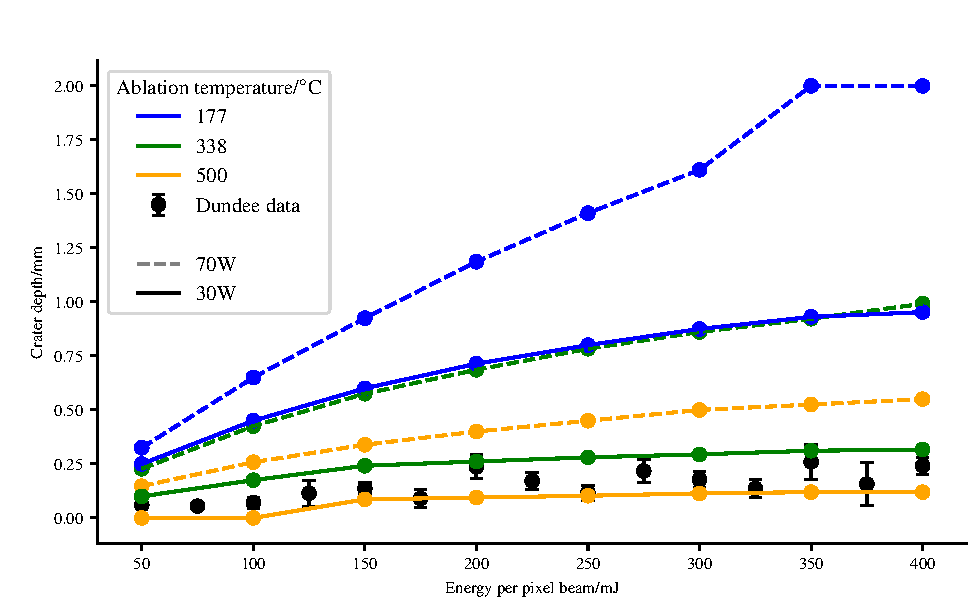
\includegraphics[width=\columnwidth]{./ablation/images/both.pdf}
    \caption{Simulations of 30~$W$ and 70~$W$ CO$_2$ ablative laser. Crater depths as a function of pixel beam energy for various \gls{ta}'s. *placeholder until I get 70W dundee data.*}\label{fig:ta}
\end{figure}
 

\subsubsection{Investigating Thermal damage} 

As stated in~\cref{sec:coagdamage}, we use the Arrhenius damage integral in order to estimate the thermal damage due to the laser. In order to calculate the tissue damage around the ablation craters, we first transform~\cref{eqn:arrhenius} in to a summation:

\begin{align}
\Omega(t) &= \int^{t_{f}}_{t_p} Ae^{(-\tfrac{\Delta E}{RT})}d\tau \\
\Omega(t) &= \sum_{m=m_p}^{m_f} Ae^{(-\tfrac{\Delta E}{RT_{\xi}^{m}})}\Delta t\label{eqn:damagesum}
\end{align}
 
\noindent Where: 
	
	\indent $\Delta E$, $R$, $T$, and $A$ have the same meanings as before;
	
	\indent $\xi$ is the $i^{th}, j^{th}, k^{th}$ node;
	
	\indent and $m_p$ is the $p^{th}$ timestep when the $\xi^{th}$ node is above the threshold temperature.

	\medskip
	
	Using~\cref{eqn:damagesum} we can thus estimate the damage to the tissue on a voxel by voxel basis.~\Cref{fig:damfig} show how far the thermal damage extends around the ablation crater. For ease of visualisation we map 1-3 to their respective burns via the following scheme, with $\eta$ as burn severity:
	
\begin{equation}
\eta = 
     \begin{cases}
       \text{3,} &\quad \Omega \geq 10000\\
       \text{2,} &\quad 1 \leq \Omega < 10000\\
       \text{1,} &\quad 0.53 \leq \Omega < 1\\
       \text{0,} &\quad 0.0 \leq \Omega< 0.53.\\
     \end{cases}
\label{eqn:thermalbound}
\end{equation}

\begin{figure}[!h]
	\centering
	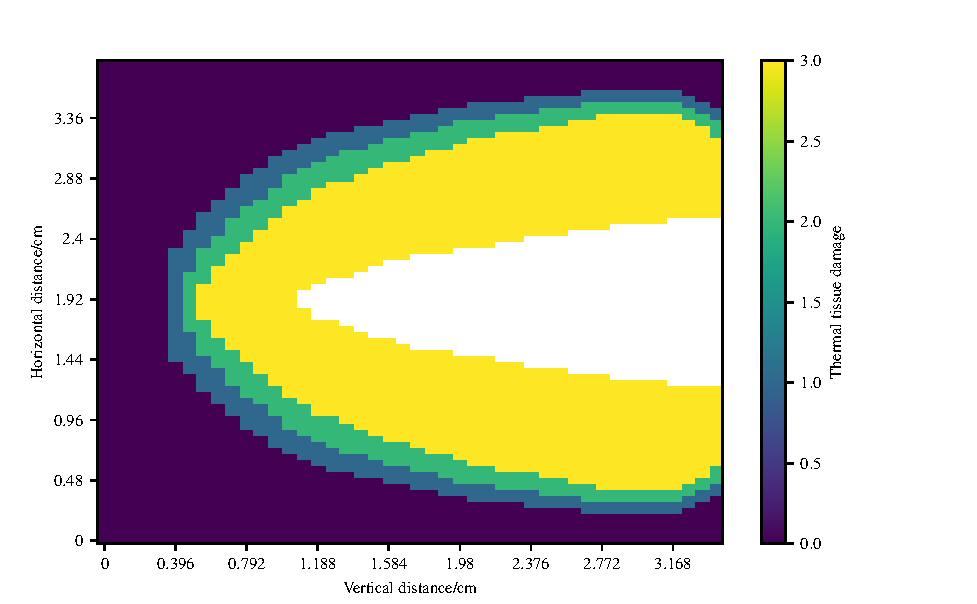
\includegraphics[width=\columnwidth]{./ablation/images/damage-slice.pdf}
	\caption{Tissue thermal damage around the ablation crater (white). Thermal tissue damage values of 3 refer to $3^{rd}$ degree burns, 2 to $2^{nd}$, and 1 to $1^{st}$ degree burns respectively. P is the power in Watts, $T_a$ is the ablation temperature in Kelvin, and $E_p$ is the energy per pixel beam in $mJ$.}
	\label{fig:damfig}
\end{figure}
	
As evidenced in~\cref{fig:damfig}, the thermal damage zone extends for a small distance around the ablation crater, due to the diffusion of heat into these areas. For the lower powered laser ($30~W$) there seems to be a maximum distance in how far the thermal damage extends beyond the ablation crater horizontally. \Cref{fig:horz-30} show this cut-off which appears to start around $250~mJ$.  
	
\begin{figure}[!h]
	\centering
	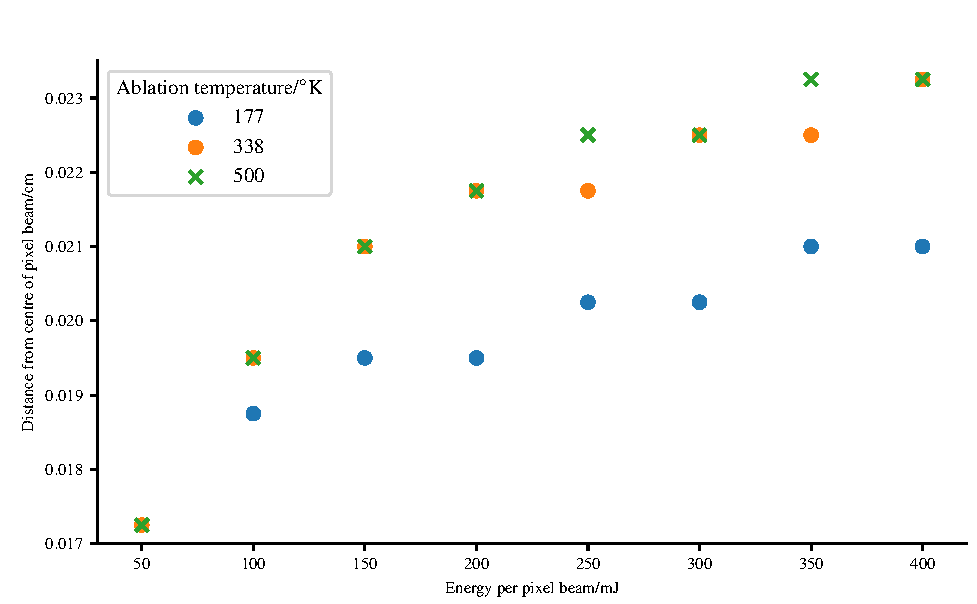
\includegraphics[width=\columnwidth]{./ablation/images/horz-30w.pdf}
	\caption{Figure shows the maximum horizontal extent of thermal damage as a function of energy per pixel beam for laser of power $30~W$. Cut-off in thermal damage appears to set in around $250~mJ$.}
	\label{fig:horz-30}
\end{figure}

In the higher powered laser ($70~W$), it appears that there is no upper cut-off for the maximum horizontal extent of thermal damage. A possible reason for this is that the simulated energies for the pixel beams were not large enough to reach the cut-off, and thus if more heat was deposited by the laser it would defuse further into the tissue.

\begin{figure}[!h]
	\centering
	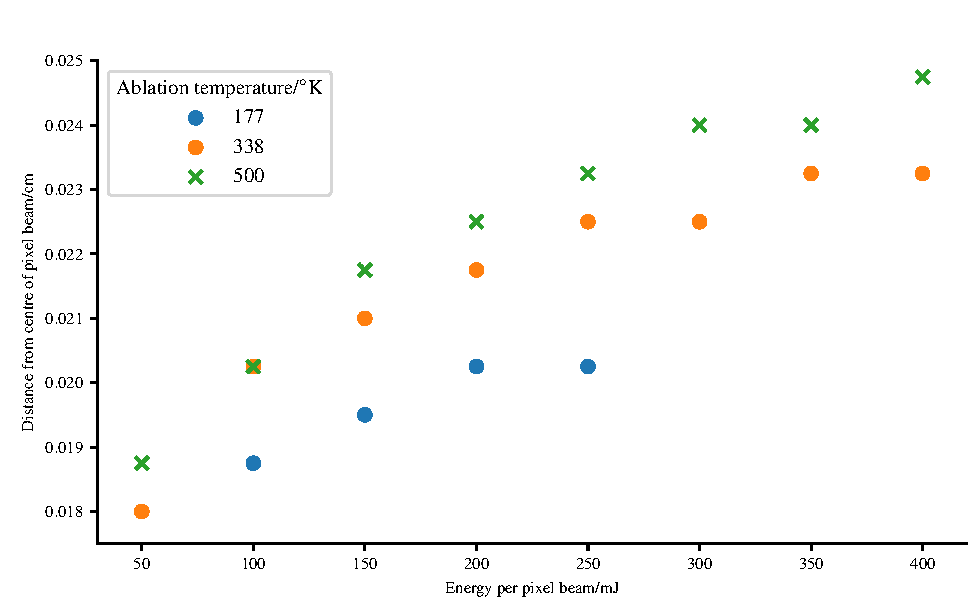
\includegraphics[width=\columnwidth]{./ablation/images/horz-70w.pdf}
	\caption{Figure shows the maximum horizontal extent of thermal damage as a function of energy per pixel beam for laser of power $70~W$. There appears to be not cut-off in the horizontal extent of the thermal damage.}
	\label{fig:horz-70}
\end{figure}

\medskip

We can also investigate the time it takes for different areas of the tissue to become thermally damaged. This can be easily achieved by saving the time each voxel passes one of the damage boundaries in~\cref{eqn:thermalbound}.~\Cref{fig:time-thres} show the minimum time taken for $1^{st}$, $2^{nd}$, and $3^{rd}$ degree burns to occur for both 30~$W$ and 70~$W$ powered lasers as a function of depth. The 70~$W$ laser shows that there is little to no time (upon the order of $0.5$~$ms$) between $1^{st}$ and $2^{nd}$ degree burns, and a maximum of $\sim$~$0.02$~$s$ between $2^{nd}$ and $3^{rd}$ degree burns.
The 30~$W$ has a larger time differential between burn classifications, with a maximum of $0.02$~$s$ between $1^{st}$ and $2^{nd}$ degree burns and a maximum of $0.2$~$s$ between $2^{nd}$ and $3^{rd}$ degree burns.
The spatial distance between burn boundaries are also drastically different between the two different powers of laser. At 70W there is virtually no difference in the boundaries for the 1st and 2nd degree burns, with a slight difference of $\sim$ $5$~$\mu m$ between the $2^{nd}$ and $3^{rd}$ degree burns. 30~$W$ the distance between $2^{nd}$ and $3^{rd}$ is $\sim 11\mu m$, and for  $1^{st}$ and $2^{nd}$ $\sim 1 \mu m$.
	
\begin{figure}
	\centering
	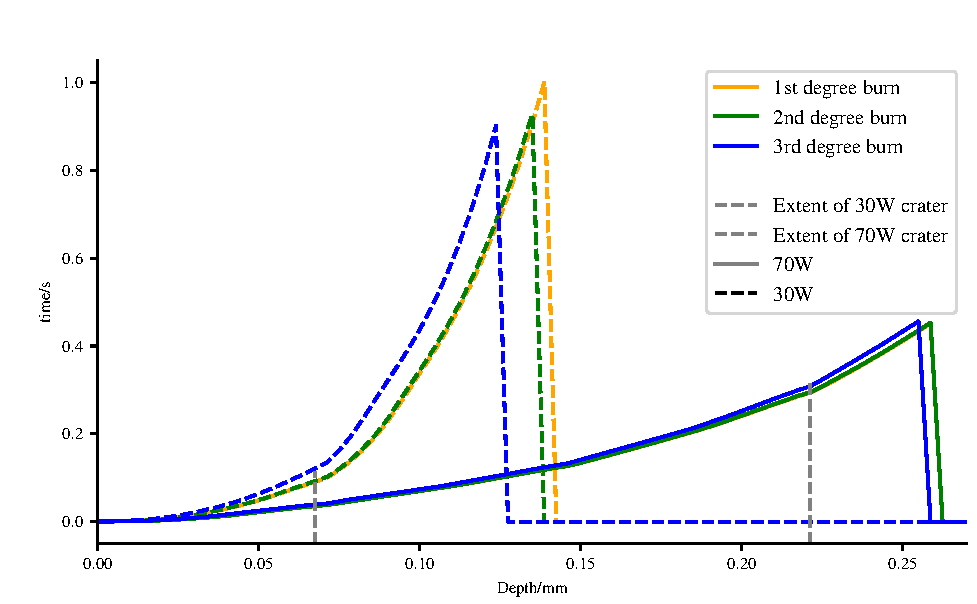
\includegraphics[width=\columnwidth]{./ablation/images/time-thres.pdf}
	\caption{Figure shows the extent of burns inflicted by the laser as a function of depth. Lines are taken from the central point of the laser beam through the tissue. Coloured dashed lines are 30W laser and solid coloured lines are 70W laser. Both data sets plotted for ablation temperature of 420~$^{\circ}C$, and pixel beam energy of 400~$mJ$}
	\label{fig:time-thres}
\end{figure}	
	
\section{Conclusion}

Using \gls{mcrt} and finite difference method, we have created a fully 3D model of photon and heat transport within tissue. This model can be used to simulate the heat deposited by laser, the ablation craters formed via high powered laser and the resultant thermal damage surrounding the ablation crater.

Our model has been fully validated against both analytical solutions and experimental results. We found that to match with experimental results that a tissue ablation temperature $T_a$ of around $420~K$ has to be adopted.

The simulations allow us to predict for a given laser power and pulse length, how much thermal damage is caused in the tissue, and how deep an ablation crater that will form.
